\chapter{Arquitectura}

En este capitulo se dará cuenta de la arquitectura digital de los módulos implementados de manera exclusiva para este trabajo. Pero antes de eso, es pertinente especificar el formato que tienen los datos en su paso por la interfaz de acceso a la cabecera.

Todas las palabras de cada paquete que ingresa a la interfaz de acceso a la cabecera, lleva anexa un campo de 8 bits que contienen el valor de los campos de control que corresponden a esa palabra y además 3 bits libres en donde se escribirá la etiqueta con los resultados de lo procesado en el software. En la figura \ref{fig:datocontrol}  es posible ver el valor de cada uno de estos campos.

\begin{figure}[H]
  \centering
	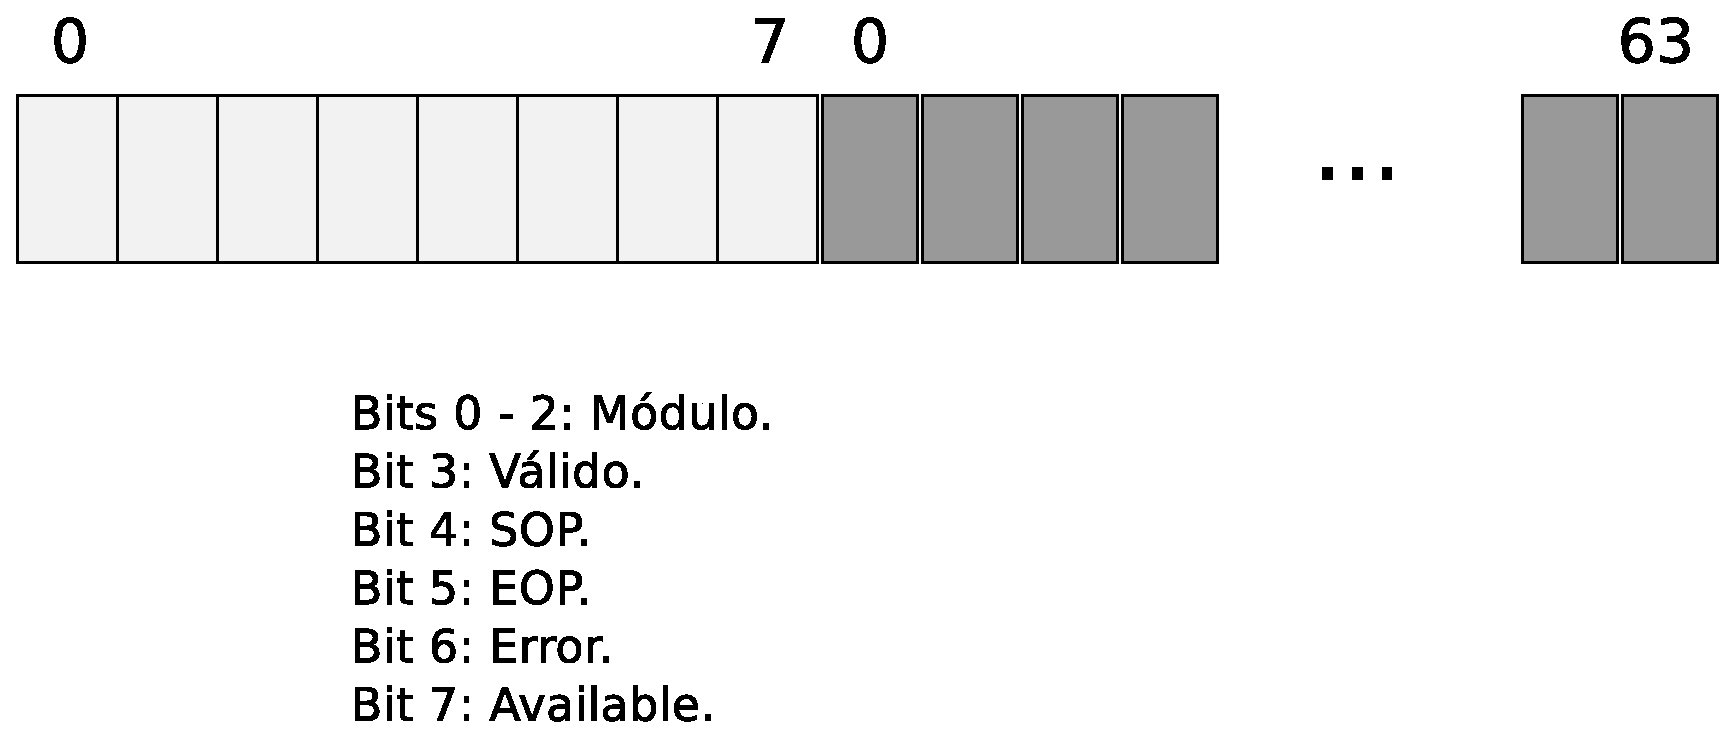
\includegraphics[scale=0.40]{3-arquitectura/graf/datocontrol.eps}
  \caption{Bits de Control anexados a cada palabra}
  \label{fig:datocontrol}
\end{figure}

Para ilustrar el funcionamiento del sistema se puede observar en la figura~\ref{fig:interfaz1} el estado del identificador de interfaz de salida en cada uno de los módulos que integran la interfaz de acceso a la cabecera.

\begin{figure}[H]
  \centering
	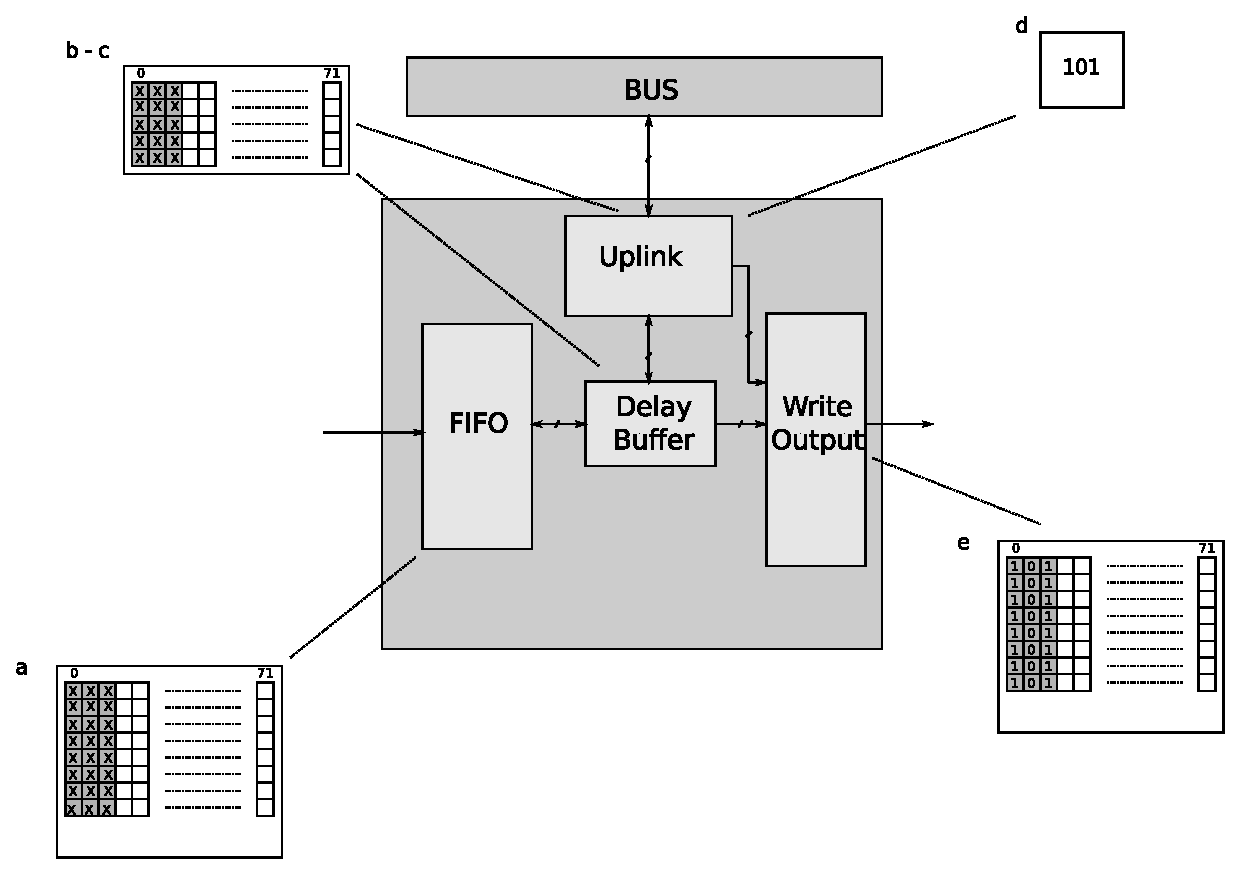
\includegraphics[scale=0.60]{3-arquitectura/graf/moduloexp.eps}
  \caption{Estado del campo de control}
  \label{fig:interfaz1}
\end{figure}

\section{Generador}

Con la intención de simplificar el desarrollo y el futuro debugging del proyecto se reemplazo la interfaz de red por un generador de paquetes.

\begin{figure}[H]
  \centering
	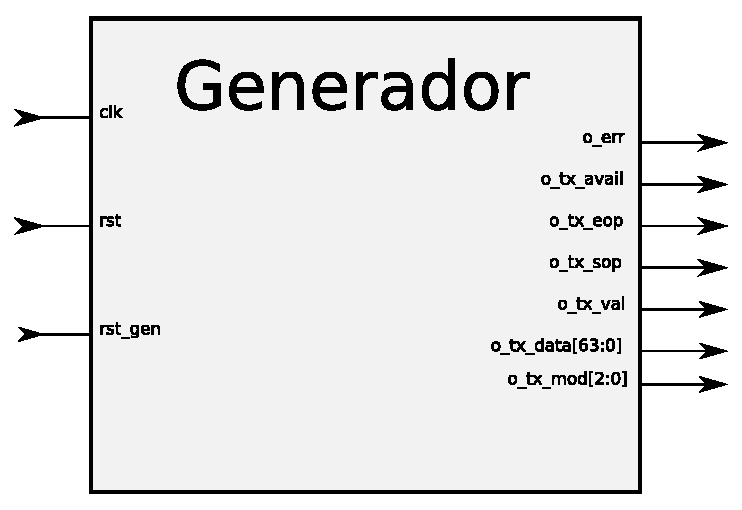
\includegraphics[scale=0.50]{3-arquitectura/graf/bloqgenerador.eps}
  \caption{módulo generador de Paquetes}
  \label{fig:gen}
\end{figure}


El mismo cuenta con las siguientes capacidades:

\begin{itemize}
	\item Permite iniciar la generación de paquetes desde un interruptor externo.
	\item Es posible parametrizar la distancia, en ciclos de clock, entre la generación de un paquete y el siguiente.
	\item Puede generar una cantidad variable de paquetes, con valores diferentes en todos sus campos.
	\item Mantiene un contador global de la cantidad de paquetes generados y lo imprime en la última palabra del Payload de cada uno.
\end{itemize}

Este módulo es una versión adaptada y mejorada del generador usado en otro proyecto integrador\cite{spaz} desarrollado en el Laboratorio de Comunicaciones Digitales.

\section{Interfaz de Acceso a la Cabecera}
En base a la figura~\ref{fig:inter}, se pasará a describir de manera detallada la estructura y el funcionamiento de cada uno de los módulos que componen la Interfaz de Acceso a la Cabecera. 

\subsection{FIFO}
Se trata de una FIFO estándar, basada en un código disponible en OpenCores\cite{fifo}, que soporta palabras de 72 bits, 64 del paquete, 5 de control y 3 del identificador de interfaz de salida. Como capacidad extra se le agregó un mecanismo para controlar la integridad de los paquetes que ingresan, aceptando solo los que pueden ser almacenados completamente en la memoria interna. 

\begin{figure}[H]
  \centering
	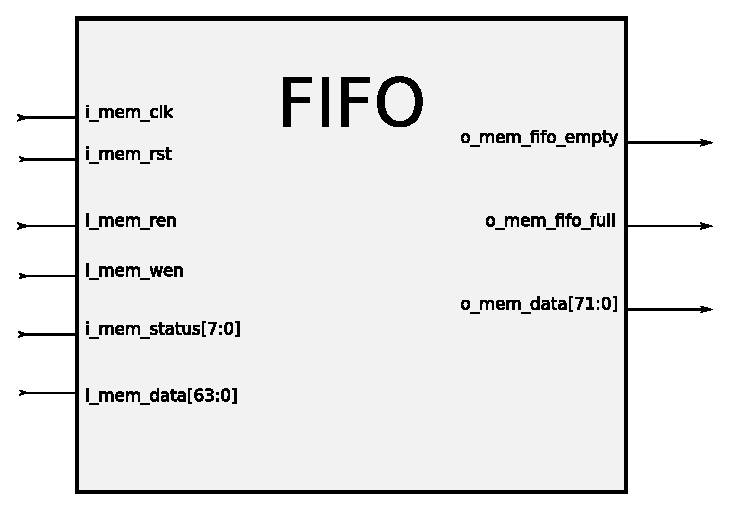
\includegraphics[scale=0.50]{3-arquitectura/graf/bloqfifo.eps}
  \caption{FIFO}
  \label{fig:gen}
\end{figure}

\subsection{Delay Buffer}
Este módulo fue desarrollado íntegramente para este proyecto y está compuesto por un registro de desplazamiento interno, que cuenta, en esta configuración, con 8 posiciones de 72 bits cada una. Su función principal es detectar la llegada de un paquete a la FIFO, cargar 5 palabras correspondientes a la cabecera, y enviar una copia a Uplink. Luego, cuando el microprocesador termina su procesamiento, continua leyendo la FIFO y transfiere el resto del paquete. Este módulo permite, además, desacoplar el flujo de datos de la comunicación con el Microprocesador.

La implementación de este módulo está formada por la máquina de estados que se muestra en la figura~\ref{fig:dbstate}.

\begin{figure}[H]
  \centering
	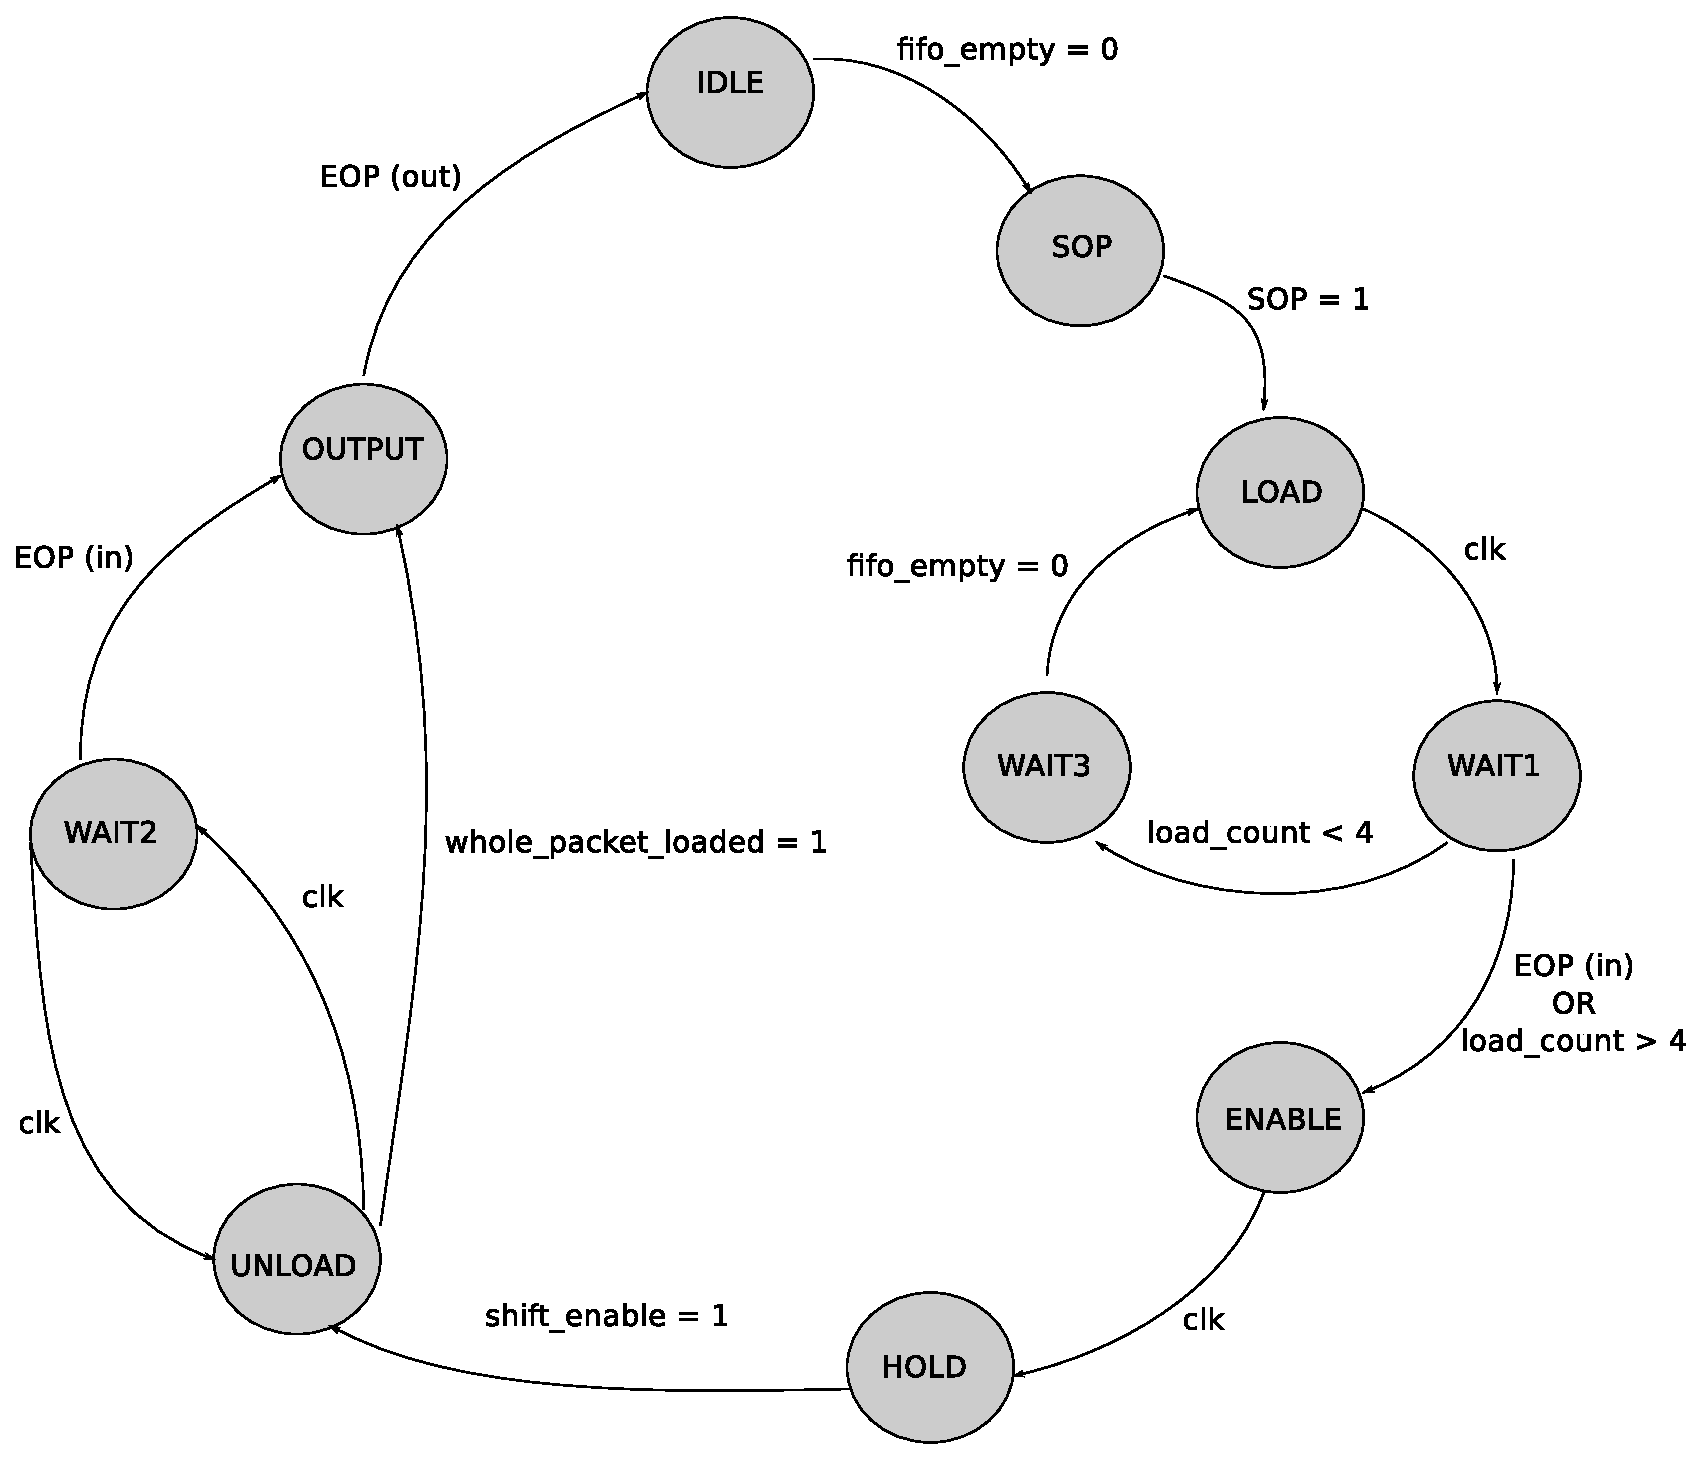
\includegraphics[scale=0.50]{3-arquitectura/graf/estdelaycompleto.eps}
  \caption{Máquina de estados de Delay Buffer}
  \label{fig:dbstate}
\end{figure}

\begin{itemize}
	\item IDLE: es el estado inicial en el que se encuentra la máquina. Cuando se detecta la presencia de datos en la FIFO pasa al estado SOP.
	\item SOP: este estado es el encargado de validar la integridad de los paquetes, permitiendo iniciar el proceso sólo cuando lo que hay en la entrada del bus de datos es un indicador de Inicio de Paquete (SOP)
	\item LOAD, WAIT1, WAIT3: estos tres estados se alternan para ir sacando de la FIFO las 5 palabras correspondientes a la cabecera. Estos implementan además mecanismos para manejar cabeceras mas pequeñas.
	\item ENABLE, HOLD: son los estados que se encargan de poner a disposición de Uplink la Cabecera completa y quedar a la espera de los resultados.
	\item WAIT2, UNLOAD: estos estados se encargan de extraer de la FIFO las palabras restantes del paquete desplazando los espacios de memoria ya cargados. 
	\item OUTPUT: se encarga de vaciar el registro de desplazamiento llenándolo de ceros a medida que se va poniendo las palabras del paquete a la salida, en caso que no hubiera nuevos paquetes disponibles, de lo contrario el proceso se repite.
\end{itemize}

La ubicación de los datos en el registro de desplazamiento interno es representativo del funcionamiento del sistema y se muestra gráficamente en las figura~\ref{fig:regdata}
\begin{figure}[H]
  \centering

	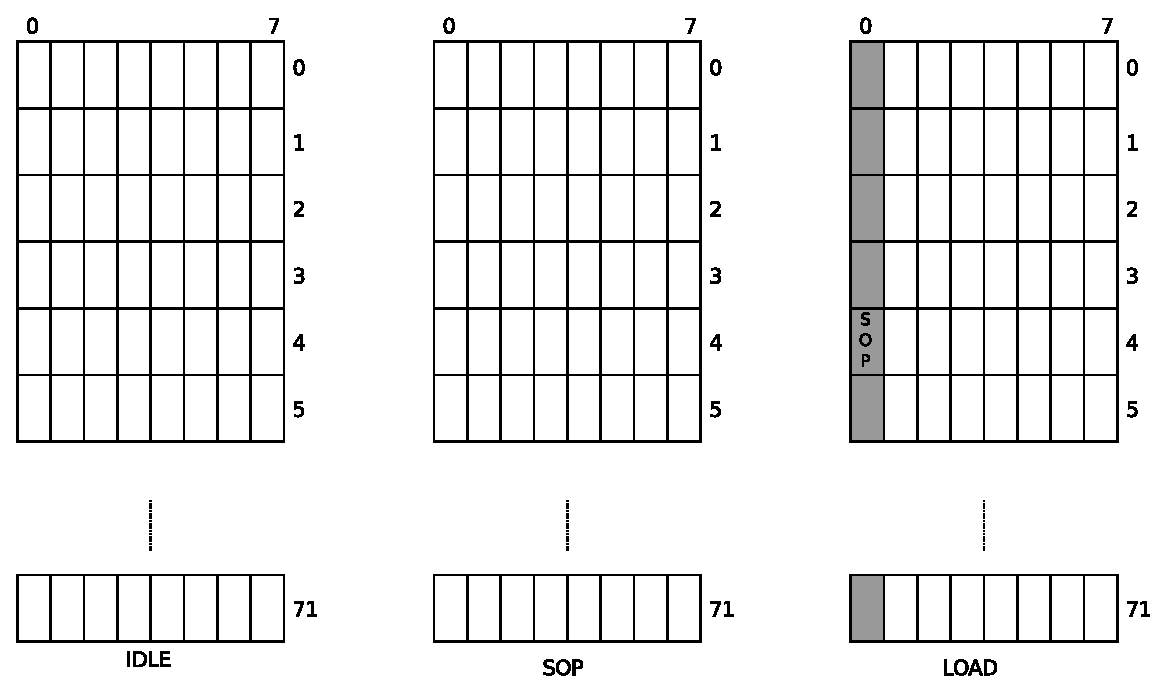
\includegraphics[scale=0.70]{3-arquitectura/graf/regdespl01.eps}


   \hspace{1\linewidth}
	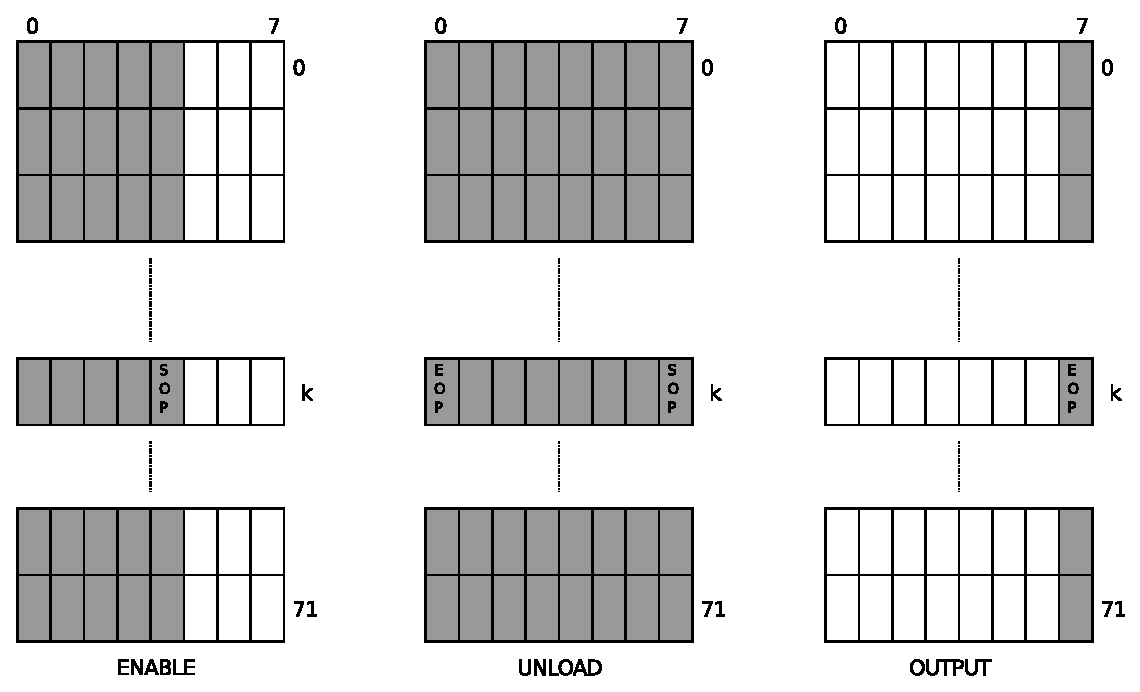
\includegraphics[scale=0.70]{3-arquitectura/graf/regdespl02.eps}



  \caption{Datos en el Registro de desplazamiento en cada estado }
  \label{fig:regdata}
\end{figure}




A continuación se presentan las señales que integran el módulo, con su correspondiente descripción:

\begin{figure}[H]
  \centering
	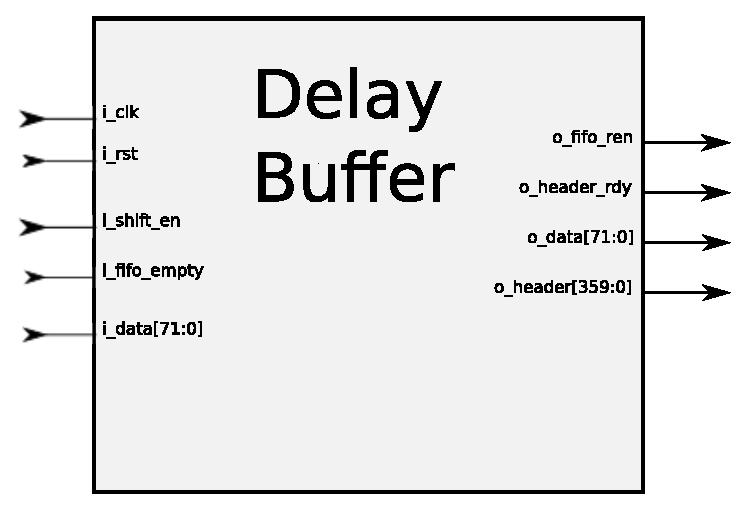
\includegraphics[scale=0.60]{3-arquitectura/graf/bloqdelaybuffer.eps}
  \caption{Delay Buffer}
  \label{fig:dbuffer}
\end{figure}


\begin{table}
	\begin{tabular}{|c|c|p{9cm}|} \hline
\rowcolor[gray]{0.1} \textcolor{white}{Nombre} & \textcolor{white}{Activo} & \textcolor{white}{Descripción}\\ \hline
\rowcolor[gray]{0.75} i\_data[71:0]	& N/A & Palabra de 72 bits que viene de la FIFO\\ \hline
\rowcolor[gray]{0.75} i\_shift\_en & High & Indica la disponibilidad de los resultados de la clasificación\\ \hline
\rowcolor[gray]{0.75} i\_fifo\_empty & Low & Señala la presencia de datos en la FIFO\\ \hline
\rowcolor[gray]{0.9} o\_data[71:0] & N/A & Salida conectada a la última posición del registro de desplazamiento\\ \hline
\rowcolor[gray]{0.9} o\_header[359:0] & N/A & Bus interno por el que pueden transferirse las 5 palabras de la cabecera en un solo ciclo\\ \hline
\rowcolor[gray]{0.9} o\_header\_rdy & High & Indica la disponibilidad de la cabecera en o\_header \\ \hline
\rowcolor[gray]{0.9} o\_fifo\_ren & High & Indica a la FIFO que se requiere una palabra nueva\\ \hline
 i\_clk & N/A & Señal de Reloj\\ \hline
 i\_rst & High & Reset\\ \hline
	\end{tabular}
	\caption{Señales de Delay Buffer}
	\label{tab:sigdb}
\end{table}


\subsection{Uplink}
El módulo Uplink gestiona la comunicación entre el procesador y el resto de los componentes de la Interfaz de acceso a la cabecera. Esta configurado para trabajar con las señales del bus Avalon (Apéndice B) de manera tal que en caso de que se desee portar esta interfaz para interactuar con otro tipo de bus, solo es necesario modificar este bloque.

Se prepararon dos versiones de Uplink; Una que transfiere al procesador la cabecera completa en 15 palabras de 32 bits y otra que solo envía una palabra de 32 bits correspondiente a la IP Destino. Ambas se ilustran en la figura~\ref{fig:up151}.

\begin{figure}[H]
  \centering
   \subfloat[15 palabras]{
	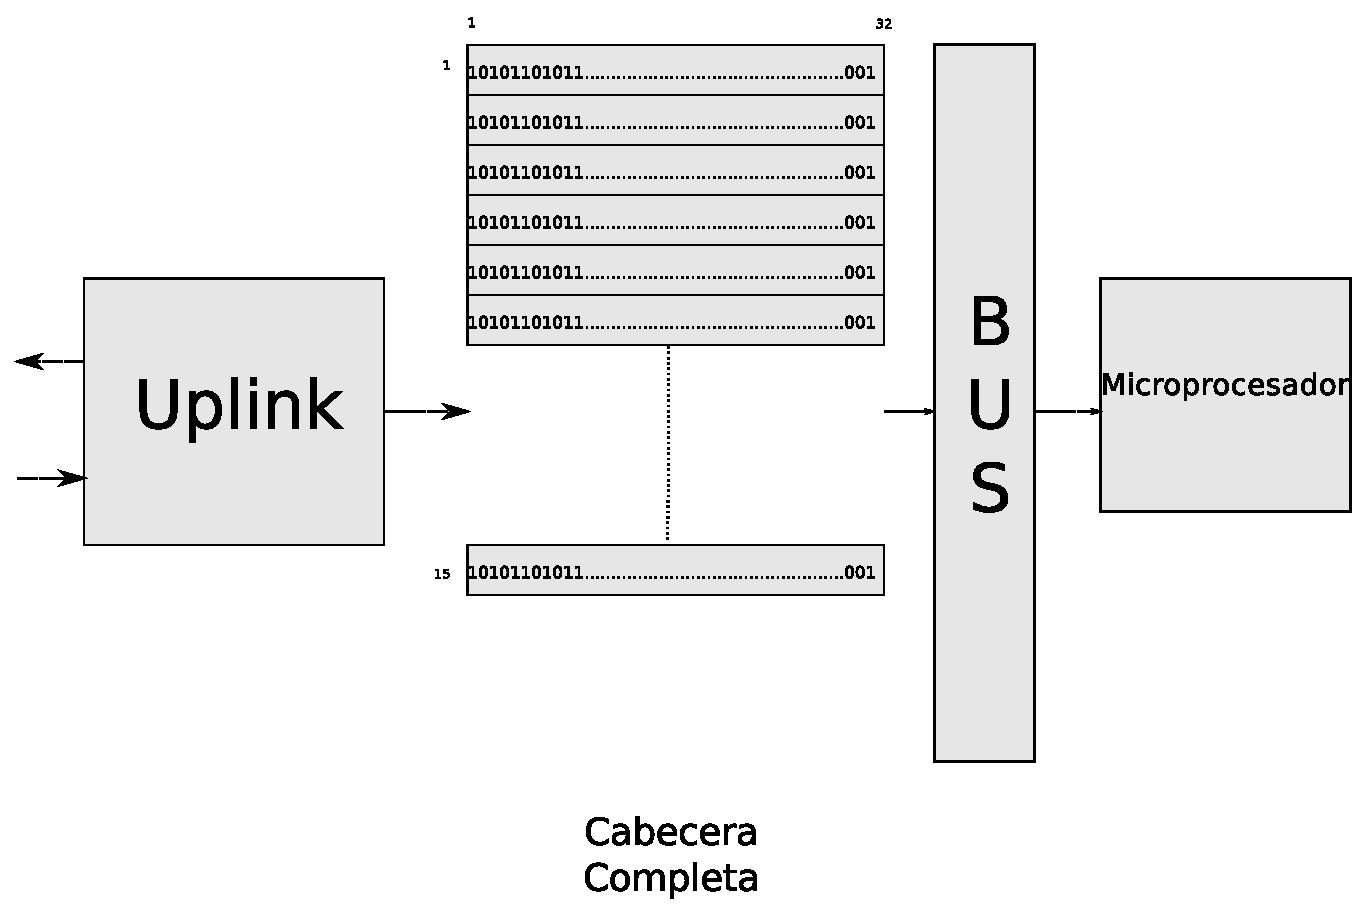
\includegraphics[scale=0.40]{3-arquitectura/graf/15pal.eps}
	        \label{fig:up151:a}         
    }

    \subfloat[1 palabra]{
        \label{fig:up151:b}         %% Etiqueta para la primera subfigura
	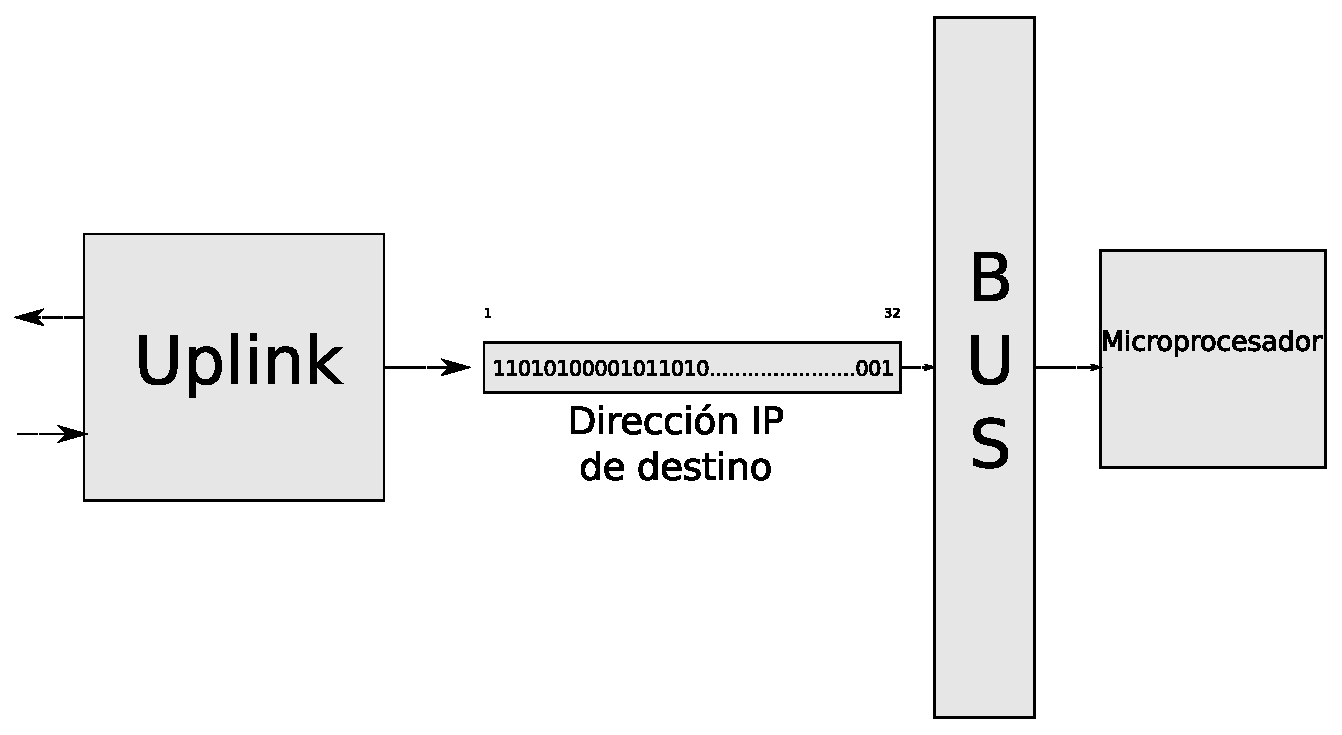
\includegraphics[scale=0.40]{3-arquitectura/graf/1pal.eps}}
   \hspace{0.1\linewidth}
  \caption{Diferentes Versiones de Uplink }
  \label{fig:up151}
\end{figure}

Este módulo implementa la máquina de estados que se puede ver en la figura~\ref{fig:inter} y se describe a continuación:

\begin{figure}[H]
  \centering
	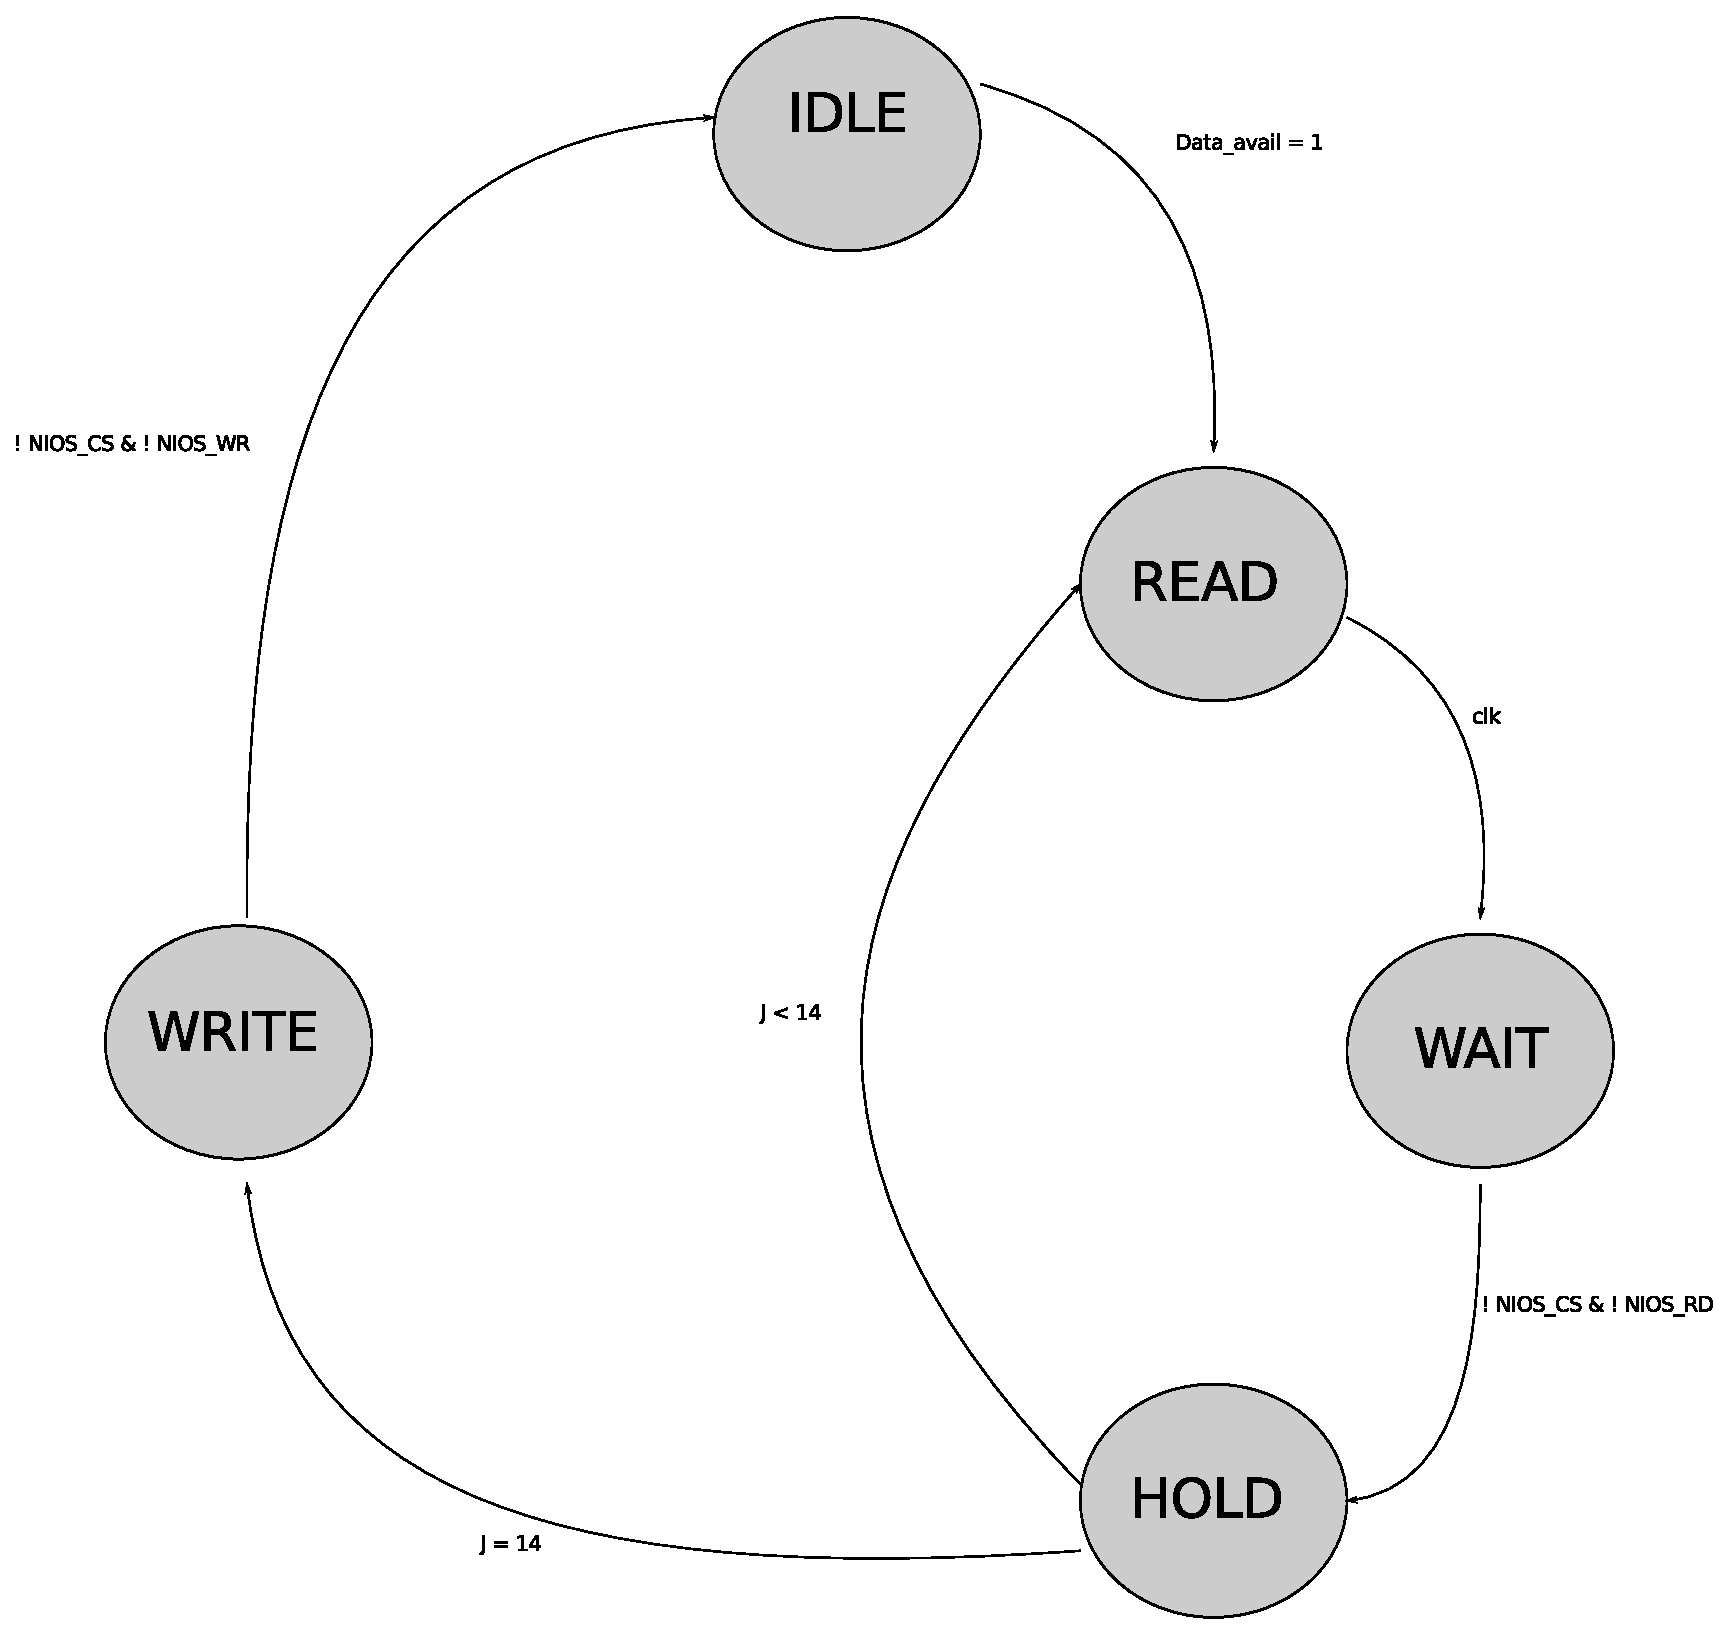
\includegraphics[scale=0.45]{3-arquitectura/graf/estuplinkcompleto.eps}
  \caption{Uplink}
  \label{fig:estuplink}
\end{figure}

\begin{itemize}
	\item IDLE: es el estado inicial en el que se encuentra la máquina, hasta que recibe la confirmación de que la cabecera esta disponible.
	\item READ,HOLD,WAIT: estos estados se alternan para interrumpir y transmitir 1 o 15 palabras de 32 bits al procesador, según el caso.
	\item WRITE: es el estado encargado de esperar que el procesador envié los resultados, para luego dar aviso a los otros componentes de la disponibilidad de los mismos.
\end{itemize}

En la tabla que sigue se pueden ver las señales que componen el módulo con su correspondiente descripción:

\begin{figure}[H]
  \centering
	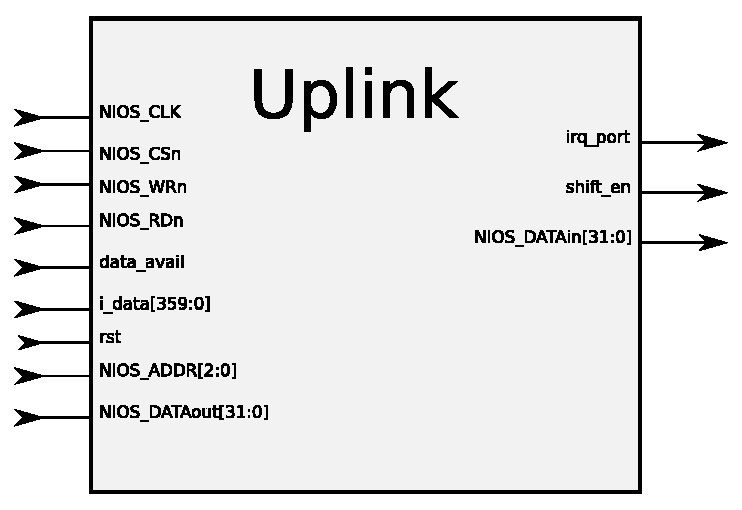
\includegraphics[scale=0.55]{3-arquitectura/graf/bloquplink.eps}
  \caption{Uplink}
  \label{fig:bloquplink}
\end{figure}
	
\begin{table}
	\begin{tabular}{|c|c|c|p{6cm}|} \hline
\rowcolor[gray]{0.1} \textcolor{white}{Nombre} & \textcolor{white}{I/O} & \textcolor{white}{Activo} & \textcolor{white}{Descripción}\\ \hline
\rowcolor[gray]{0.75} i\_data[359:0] & Input & N/A & Bus interno por donde Delay Buffer envía la cabecera entera en un ciclo\\ \hline
\rowcolor[gray]{0.75} data\_avail & Input & High & Señala la disponibilidad de la Cabecera\\ \hline
\rowcolor[gray]{0.75} NIOS\_DATAout[31:0] & Input & N/A & Bus de datos desde el procesador\\ \hline
\rowcolor[gray]{0.75} NIOS\_ADDR[2:0] & Input & N/A & Bus de direcciones Avalon\\ \hline
\rowcolor[gray]{0.75} NIOS\_CSn & Input & Low & Señal Avalon que indica que se está trabajando con este componente\\ \hline
\rowcolor[gray]{0.75} NIOS\_RDn & Input & Low & Indica que el procesador está leyendo los datos presentes en NIOS\_DATAin \\ \hline
\rowcolor[gray]{0.75} NIOS\_WRn & Input & Low & Señala la disponibilidad de datos en NIOS\_DATAout\\ \hline
\rowcolor[gray]{0.9} NIOS\_DATAin[31:0] & Output & N/A & Bus de datos de entrada al procesador\\ \hline
\rowcolor[gray]{0.9} shift\_en & Output & High & Avisa a los otros componentes que ya están listos los resultados\\ \hline
\rowcolor[gray]{0.9} irq\_port & Output & High & Señal de Interrupción\\ \hline
 NIOS\_CLK, & Input & N/A & Señal de Reloj\\ \hline
 rst & Input & High & Reset\\ \hline
	\end{tabular}
	\caption{Señales de Uplink}
	\label{tab:sigup}
\end{table}

\newpage

\subsection{Write output}

Este módulo es el que se encarga de tomar el resultado emitido por el microprocesador y de colocarlo en los campos de control anexos a cada una de las palabras del paquete. Se puede ver en la figura~\ref{fig:inter} el diagrama de estados en base al cual esta implementado este módulo, y se describe cada estado a continuación:

\begin{figure}[H]
  \centering
	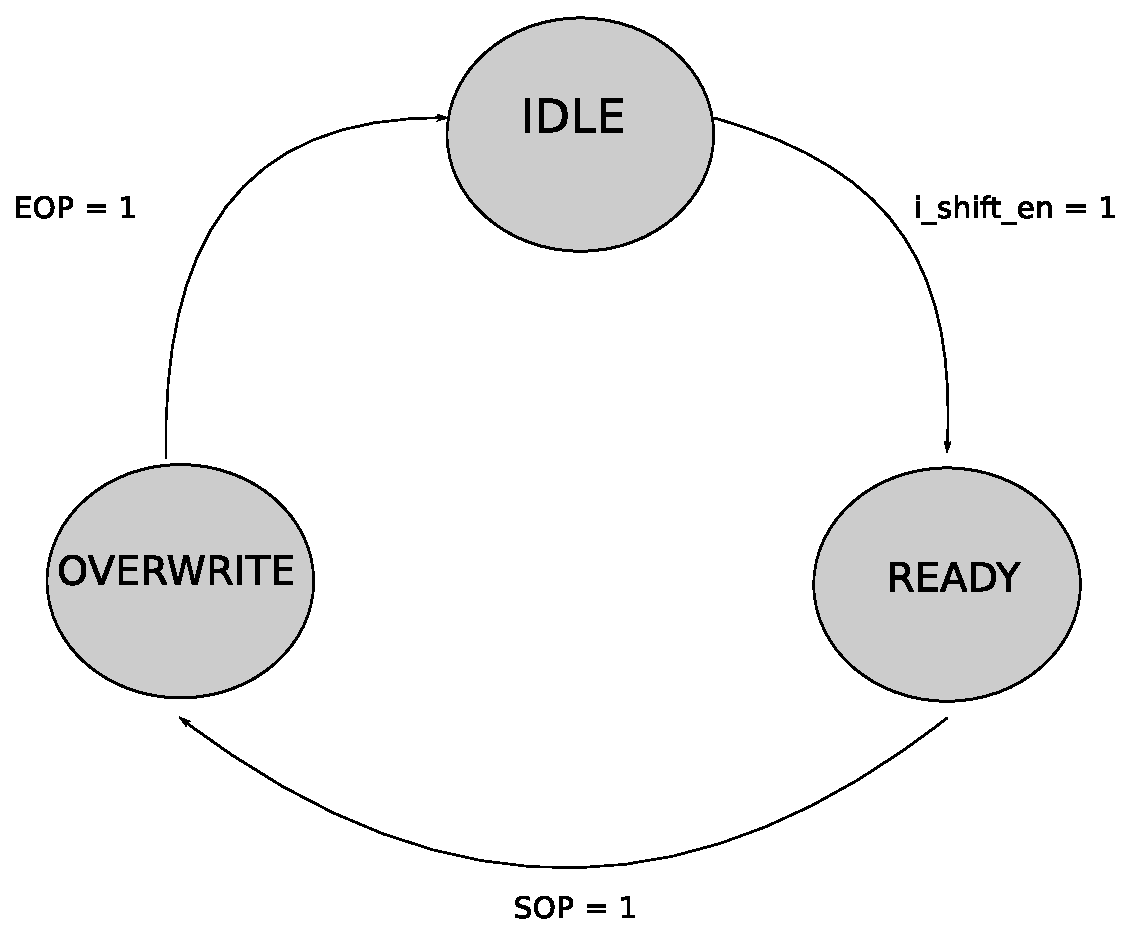
\includegraphics[scale=0.45]{3-arquitectura/graf/estwritecompleto.eps}
  \caption{Diagrama de Estados de Write Output}
  \label{fig:estuplink}
\end{figure}

\begin{itemize}
	\item IDLE: es el estado inicial en el que se encuentra la máquina, hasta que recibe la confirmación de que los resultados están disponibles.
	\item READY: espera que Delay Buffer le transmita la palabra correspondiente a un SOP. 
	\item OVERWRITE: escribe el resultado en el Tag adjunto a cada palabra hasta que encuentra la palabra correspondiente a un EOP. 
\end{itemize}

A continuación se detalla las señales de Entrada/Salida del módulo y su función:

\begin{figure}[H]
  \centering
	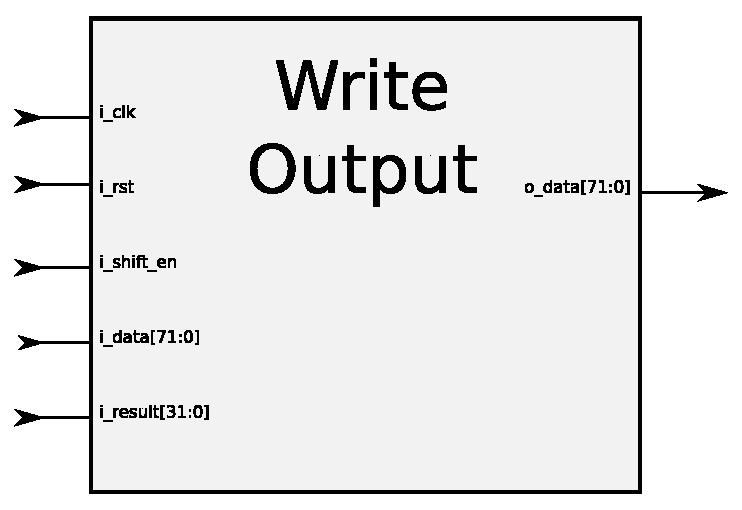
\includegraphics[scale=0.55]{3-arquitectura/graf/bloqwrite.eps}
  \caption{Uplink}
  \label{fig:bloquplink}
\end{figure}
	

\begin{table}
	\begin{tabular}{|c|c|p{9cm}|} \hline
\rowcolor[gray]{0.1} \textcolor{white}{Nombre} & \textcolor{white}{Activo} & \textcolor{white}{Descripción}\\ \hline
\rowcolor[gray]{0.75} i\_data[71:0]	& N/A & Palabra de 72 bits proveniente Delay Buffer\\ \hline
\rowcolor[gray]{0.75} i\_shift\_en & High & Indica la disponibilidad de los resultados de la clasificación\\ \hline
\rowcolor[gray]{0.75} i\_result[32:0] & N/A! & Esta conectado a NIOS\_DATAout y conserva lo escrito por el procesador mientras i\_shift\_en esta activa \\ \hline
\rowcolor[gray]{0.9} o\_data[71:0] & N/A & Salida de las palabras con el resultado anexo\\ \hline
 i\_clk & N/A & Señal de Reloj\\ \hline
 i\_rst & High & Reset\\ \hline
	\end{tabular}
	\caption{Señales de Write Output}
	\label{tab:sigwo}
\end{table}




